\section{Appendix: Handwritten records of the experiment}
\label{sec:records}
%    \includegraphics[width=\linewidth]{appendix/}
%\clearpage


\section{Appendix: Plots for measurement of different gratings.}
\label{sec:appendix_gratings_plots}
\begin{figure}
    \centering
    \begin{subfigure}[b]{\mpltw}
        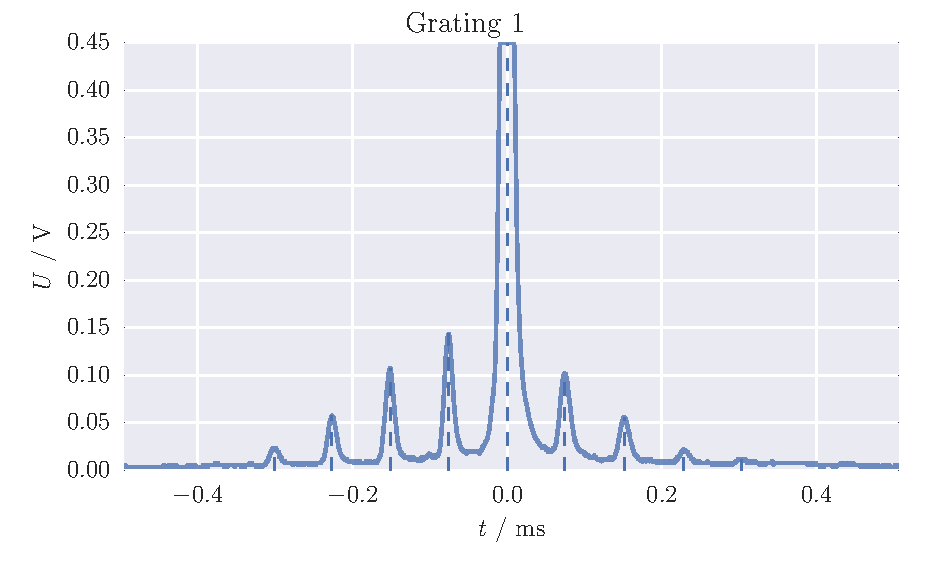
\includegraphics[width=\textwidth]{figures/gratings_maxi1.pdf}
        \caption{Grating 1}
        \label{fig:gratings_maxi1}
    \end{subfigure}\quad
    \begin{subfigure}[b]{\mpltw}
        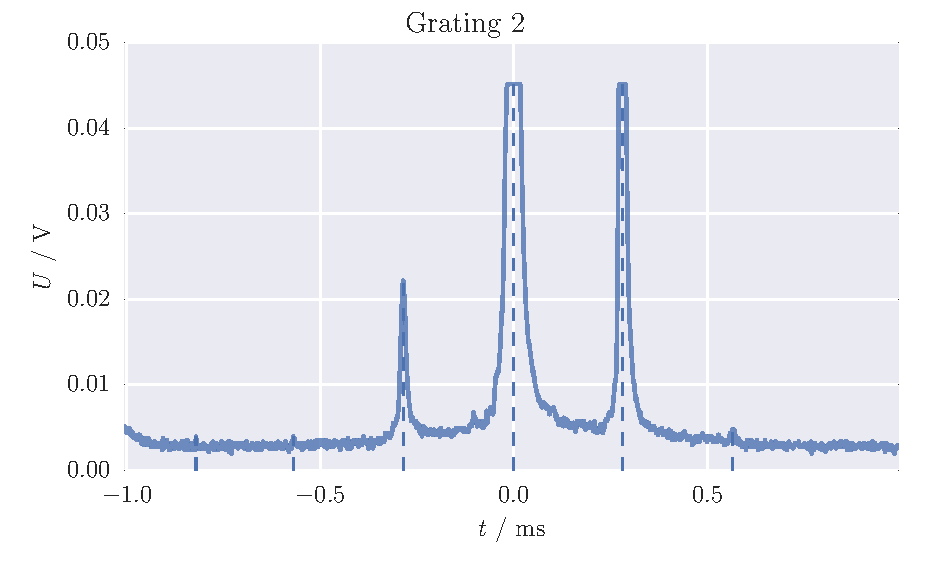
\includegraphics[width=\textwidth]{figures/gratings_maxi2.pdf}
        \caption{Grating 2}
        \label{fig:gratings_maxi1}
    \end{subfigure}
    \begin{subfigure}[b]{\mpltw}
        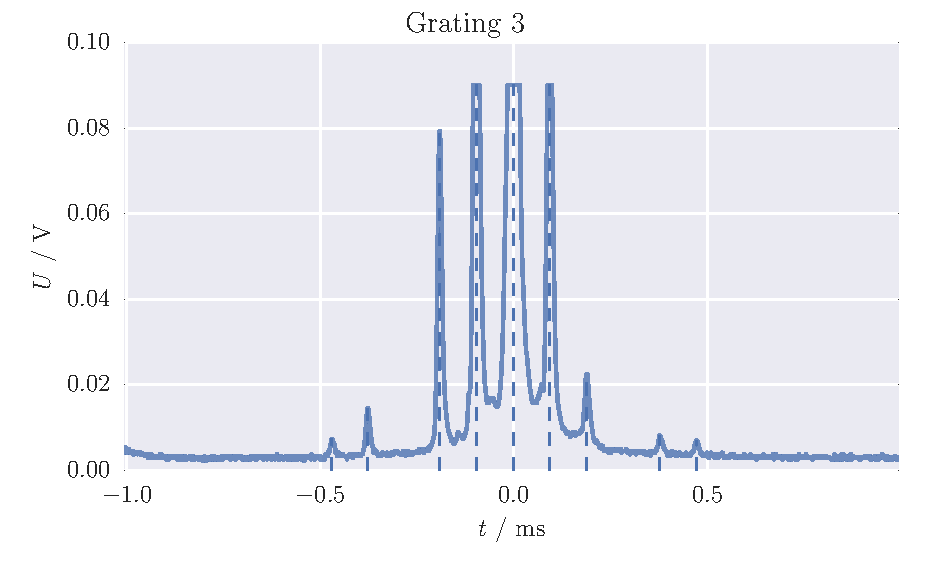
\includegraphics[width=\textwidth]{figures/gratings_maxi3.pdf}
        \caption{Grating 3}
        \label{fig:gratings_maxi1}
    \end{subfigure}\quad
    \begin{subfigure}[b]{\mpltw}
        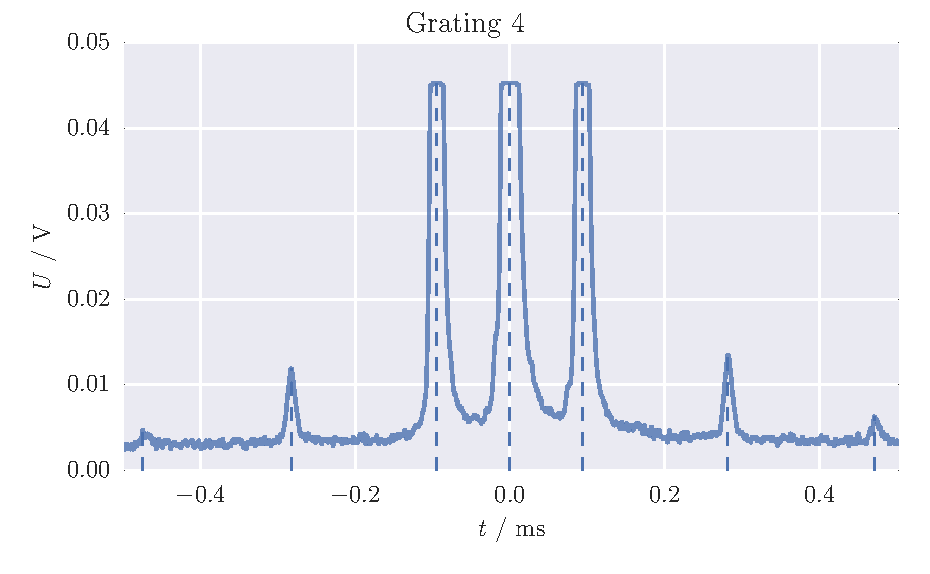
\includegraphics[width=\textwidth]{figures/gratings_maxi4.pdf}
        \caption{Grating 4}
        \label{fig:gratings_maxi1}
    \end{subfigure}
    \begin{subfigure}[b]{\mpltw}
        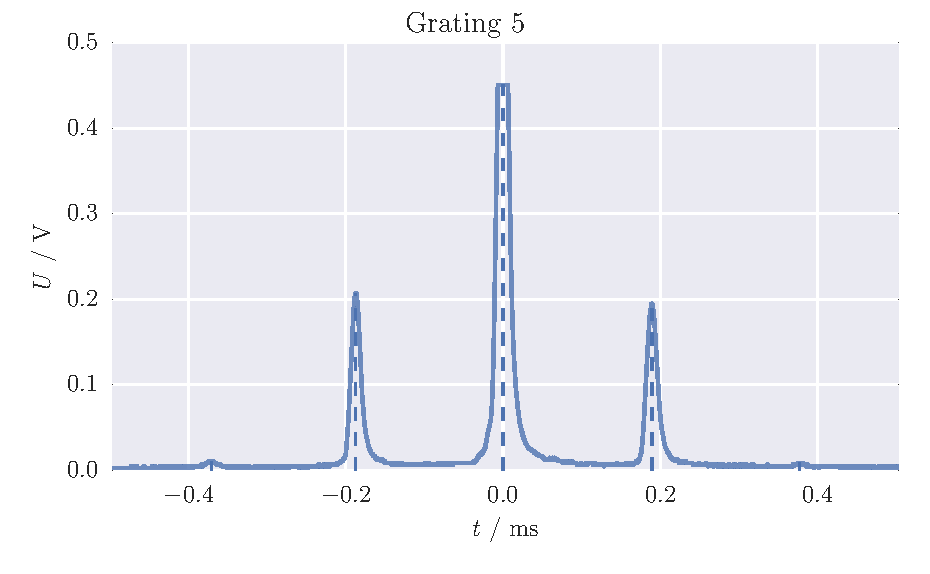
\includegraphics[width=\textwidth]{figures/gratings_maxi5.pdf}
        \caption{Grating 5}
        \label{fig:gratings_maxi1}
    \end{subfigure}
    \caption{
        Measured spectra of gratings with maxima numerically found (shown as broken 
            lines). The maximum of zeroth order is not used in the analysis. 
        }
    \label{fig:gratings_maxima}
\end{figure}
